\section{Einleitung}
\label{sec:einleitung}

Heutzutage haben Webdienste einen hohen Stellenwert im Internet. Sie sind häufig ein essenzieller Bestandteil von Anwendungen und werden durch eine \textit{Representation State Transfer} (REST)-Schnittstelle für Anwender und Entwickler angeboten. Auch das Internet of Things (IoT) bekommt mit fortschreitender Zeit eine wichtigere Rolle in der Entwicklung von Anwendungen, wie zum Beispiel Hausautomatisierung oder smarte Energieverwaltung.

Um die REST-Architektur auch für eingeschränkte Geräte anzubieten, wurde mit \textit{Constrained RESTful Environments} (CoRE) eine geeignete Form gebildet. Somit können solche Geräte, wie zum Beispiel 8-Bit-Mikrocontroller mit begrenztem Arbeitsspeicher und Readonly-Memory, und Netzwerke, wie zum Beispiel \textit{IPv6 over Low-Power Wireless Area Networks (6LoWPANs)}, solche Architekturen verwenden und realisieren. Damit eine Fragmentierung von Nachrichten in solchen Netzwerken so wenig wie möglich auftritt, wird im Constrained Application Protocol (CoAP) ein so niedriger Nachrichten-Overhead wie möglich angestrebt.

Mit CoAP wurde die Entwicklung eines generischen Webprotokolls für die speziellen Anforderungen dieser eingeschränkten Umgebungen, insbesondere mit Hauptaugenmerk auf Energie-, Gebäudeautomatisierungs- und andere Machine-to-Machine (M2M) Anwendungen. Dabei sollte CoAP keine komprimierte Abwandlung von HTTP sein, sondern vielmehr eine Submenge von HTTP mit Verwendung von REST, die für M2M-Szenarien optimiert ist. Somit könnte CoAP leicht dazu verwendet werden, einfache HTTP-Schnittstelle in ein kompaktes Protokoll überzuführen, jedoch bietet CoAP Funktionen die speziell für Machine-to-Machine Anwendungen eine Verwendung finden. Diese Funktionen sind:
\begin{itemize}
    \item Eingebaute Entdeckung von, im Netzwerk, angebotenen Services und Ressourcen.
    \item Mutlicast-Unterstützung.
    \item Asynchronen Nachrichtenaustausch.
\end{itemize}

\subsection{Constrained Application Protocol (CoAP)}
\label{subsec:constrained-application-protocol}
Das Constrained Application Protocol, abgekürzt CoAP, ist ein Internetprotokoll, das speziell für M2M Anwendungen, wie zum Beispiel smarte Energieverwaltung oder Hausautomatisierung (Internet of Things (IoT)), entwickelt wurde. Dabei bietet das Protokoll ein REST-ähnliches Interface für Mikrocontroller mit angeschlossenen Aktoren oder Sensoren (\textit{constrained nodes}) oder auch drahtlose Sensornetze (\textit{constrained networks}) an. Die sogenannten \textit{nodes} besitzen meist einen angeschlossenen 8-Bit-Mikrocontroller, der nur eine kleine begrenzte Menge an Arbeitsspeicher (RAM) und Readonly-Memory (ROM) beinhaltet. Bei \textit{contstrained networks}, wie z.B. \textit{IPv6 over Low-Power Wireless Area Networks (6LoWPANs)}, spielt die hohe Paketverlustrate und der für solche Netzwerke typische Datendurchsatz von wenigen 10 kbit/s eine große Rolle. CoAP ist durch den RFC 7252 \autocite{RFC7252} spezifiziert.

Dabei bietet das \textit{Constrained Application Protocol} ein Interaktionsmodell für Anfragen und Antworten zwischen den, in der Anwendung definierten, Endpunkten an. Auch ist eine eingebaute Entdeckung von im Netzwerk angebotenen Services und Ressourcen im Protokoll definiert. Zusätzlich werden Hauptbestandteile des Internets, wie \textit{Unique Resource Identifiers} (URIs) und \textit{Internet Media Types} (zum Beispiel \textit{application/json}).

Eine Unterstützung von \textit{Multicast} ist gegeben, wie auch ein sehr geringer Mehraufwand in der Datenübertragung. Dabei wurde Wert darauf gelegt, es einfach für eingebettete Systeme zu halten.  

Zur Datenübertragung nutzt CoAP das User Datagram Protocol (UDP). Dieses unterscheidet sich zu Transmission Control Protocol (TCP) in den folgenden Punkten:
\begin{itemize}
    \item kein Sitzungsaufbau von Sender zu Empfänger (Handshake).
    \item Stellt nicht sicher, ob alle Pakete beim Empfänger eintreffen.
    \item Geht ein Paket verloren, wird dieses nicht erneut versendet.
\end{itemize}

Die folgenden Funktionen sind ein essenzieller Bestandteil von CoAP:
\begin{itemize}
    \item Erfüllung von M2M Anforderungen in eingeschränkten Umgebungen.
    \item UDP-Verbindung mit optionaler Zuverlässigkeit, die Unicast- und Multicast Anfragen unterstützt.
    \item Asynchroner Nachrichtenaustausch.
    \item Niedriger Mehraufwand durch veränderten Header und niedrige Komplexität des Parsings.
    \item URI- und Content-Typen-Support.
    \item Einfache Proxy- und Caching-Unterstützung.
    \item Zustandsloses HTTP-Mapping das die Entwicklung von Proxys erlaubt, die den Zugriff auf CoAP Ressourcen über HTTP auf einheitliche Weise ermöglichen, oder für einfache HTTP-Schnittstellen, die alternativ über CoAP realisiert werden können.
    \item Sicherheitsmechanismen durch das Anbinden von \textit{Datagram Transport Layer Security} (DTLS).
\end{itemize}

\subsection{Begriffe in CoAP}
\label{subsec:begiffe-in-coap}

Um den Kontext innerhalb des \textit{Constrained Application Protocols} zu verstehen, werden nachfolgend die wichtigsten Begriffe in CoAP kurz erklärt:
\begin{itemize}
    \item Endpunkt (Endpoint):
    \begin{itemize}
        \item Ein Endpunkt lebt auf einen "Knoten". Ein Knoten ist vergleichbar mit dem Begriff "Host", der vorwiegend in Internetstandards Erwähnung findet.
        \item Ein Endpunkt wird durch Multiplexing-Informationen auf der Transportschicht identifiziert, die eine UDP-Portnummer und eine Sicherheitszuordnung enthalten könnte.
    \end{itemize}
    \item Ursprungsserver (Origin Server):
    \begin{itemize}
        \item Der Server, auf dem sich eine bestimmte Ressource befindet oder erstellt werden soll.
    \end{itemize}
    \item Bestätigende Nachricht (Confirmable Message):
    \begin{itemize}
        \item Einige Nachrichten benötigen eine Bestätigung des Empfängers. Diese Nachrichten werden als \textit{bestätigt} behandelt.
        \item Falls keine Pakete während der Übertragung verloren gingen, wird für jede Nachricht, die bestätigt werden muss, exakt eine Nachricht des Typs \textit{Acknowledgement} oder \textit{Reset}.
    \end{itemize}
    \item Nicht bestätigende Nachricht (Non-confirmable Message):
    \begin{itemize}
        \item Als Gegensatz zu bestätigenden Nachrichten gibt es auch Nachrichten die nicht bestätigt werden müssen.
        \item Dies trifft auf Nachrichten zu, die für bestimmte Anwendungsanforderungen häufiger wiederholt werden müssen, wie zum Beispiel wiederholtes Lesen eines Sensors.
    \end{itemize}
    \item Bestätigungsnachricht (Acknowledgement Message):
    \begin{itemize}
        \item Eine solche Nachricht bestätigt den Empfang einer bestätigenden Nachricht. Eine Bestätigungsnachricht sagt nicht aus, ob die Anfrage, die mit einer bestätigenden Nachricht versendet wurde, erfolgreich war oder nicht.
        \item Jedoch enthält die Bestätigungsnachricht auch eine sogenannte \textit{Piggybacked Response}.
    \end{itemize}
    \item Rücksetzende Nachricht (Reset message):
    \begin{itemize}
        \item Diese Nachricht sagt aus, dass eine spezifische Nachricht (\textit{Confirmable} oder \textit{Non-confirmable}) empfangen wurde, jedoch einige Teile des Nachrichtenkontextes fehlt, um die richtig zu bearbeiten.
        \item Dieses Verhalten tritt auf, wenn der zu empfangende Endpunkt neu gestartet hat und somit den Zustand vergessen hat, der zur vollständigen Interpretation der Nachricht nötig ist.
        \item Ein absichtliches Provozieren einer rücksetzenden Nachricht \textit{Reset Message}, zum Beispiel durch das Senden einer leeren bestätigenden Nachricht (\textit{Empty Confirmable Message}), kann als eine kostengünstige Prüfung der Funktionsfähigkeit eines Endpunktes verwendet werden - vergleichbar mit einem \textit{Ping}.
    \end{itemize}
    \item Piggybacked Response:
    \begin{itemize}
        \item Eine \textit{Piggybacked Response} ist direkt in eine \textit{Acknowledgement} (ACK) Nachricht inkludiert, die gesendet wird, um den Empfang der Anfrage für diese Antwort zu bestätigen.
    \end{itemize}
    \item Separate Antwort (Separate Response):
    \begin{itemize}
        \item Wenn eine \textit{Confirmable} Nachricht mit einer Anfrage mit einer \textit{Empty} Nachricht quittiert wird (z.B. weil der Server die Antwort nicht sofort hat), wird eine separate Antwort in einem separaten Nachrichtenaustausch gesendet.
    \end{itemize}
    \item Leere Nachricht (Empty Message):
    \begin{itemize}
        \item Eine Nachricht mit dem Code 0.00. Die Nachricht ist weder eine Anfrage noch eine Antwort. Es beinhaltet nur den 4-Byte-langen Kopf (\textit{header}).
    \end{itemize}
\end{itemize}

\subsection{Nachrichtenübertragung}
\label{subsec:nachrichtenuebertragung}

CoAP nutzt zur Nachrichtenübertragung UDP, um den Austausch von Nachrichten asynchron ausführen zu können. Dies wird dadurch erreicht, dass eine weitere Schicht auf UDP aufbauend eingefügt wird (siehe Bild \ref{fig:abstrakte-darstellung-der-verschiedenen-schichten}). Diese Schicht kann optional auch einen Mechanismus zur Sicherstellung des Nachrichtenaustausches beinhalten. Dabei definiert CoAP vier verschiedene Arten von Nachrichten:
\begin{itemize}
    \item bestätigende Nachricht (\textit{Confirmable Message})
    \item nicht bestätigende Nachricht (\textit{Non-confirmable Message})
    \item Bestätigungsnachricht (\textit{Acknowledgement Message})
    \item rücksetzende Nachricht (\textit{Reset Message})
\end{itemize}

Diese vier Arten stehen orthogonal zueinander, sprich:
\begin{itemize}
    \item Bestätigende und nicht bestätigende Nachrichten sind für Anfragen (\textit{requests})
    \item und rücksetzende Nachrichten oder Nachrichten, die eine Anfrage bestätigen, sind für Antworten (\textit{responses}) gedacht.
\end{itemize}

\begin{figure}[h]
    \centering
    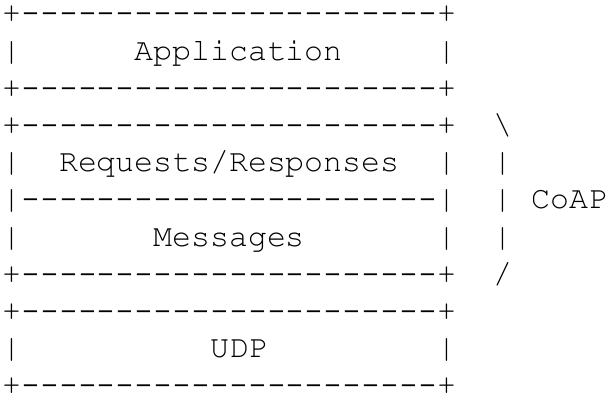
\includegraphics[width=0.5\textwidth]{abstract_layering_of_coap}
    \caption{Abstrakte Darstellung der verschiedenen Schichten}
    \label{fig:abstrakte-darstellung-der-verschiedenen-schichten}
\end{figure}

\subsubsection{Nachrichtenmodell}
\label{subsubsec:nachrichtenmodell}

Das Nachrichtenmodell des Constrained Application Protocols basiert auf den Austausch von Nachrichten über UDP. Dabei beginnt die Nachricht mit einem in der Länge fixierten Vier-Byte-Langen Kopfzeile (\textit{header}), gefolgt von einer einem optionalen Token (null bis acht Bytes lang), null oder mehr sogenannten Optionen. Diese Optionen sind vergleich mit den \textit{header fields} von HTTP. Nach den Optionen befindet sich ein sogenannter Anhang-Markierer (\textit{Payload marker}) der einem Byte mit dem Wert 0xFF (255) entspricht. Anschließend an den \textit{Payload marker} kommt der Anhang (\textit{Payload}). Dieses Format ist sowohl für Anfragen als auch für Antworten dasselbe.

Damit Nachrichten als eindeutig identifiziert werden können, wird ein sogenannter Nachrichtenbezeichner (\textit{Message ID}) verwendet. Dieser ist 16 Bit groß und erlaubt somit, bei Implementierungen mit Standardeinstellungen, bis zu 250 Nachrichten die Sekunde von einem Endpunkt zu einem anderen. Die \textit{Message ID} wird auch für die Sicherstellung des Nachrichtenaustausches (\textit{reliability}) benötigt. Dabei ist jedoch die \textit{Message ID} nur zwischen zwei Endpunkten eindeutig. Kommuniziert ein Teilnehmer mit mehreren Teilnehmern gleichzeitig, dann können die \textit{Message IDs} häufiger vorkommen. Für die eindeutige Identifizierung der Kommunikation zwischen zwei Teilnehmern wird der sogenannten Token verwendet. Dieser ist über mehrere Verbindungen hinweg eindeutig und kann als Identifikator für Verbindungen gesehen werden.

Die Sicherstellung des Nachrichtenaustausches erfolgt dadurch, dass man eine Nachricht als bestätigend (\textit{Confirmable}) markiert. Eine als \textit{Confirmable} gekennzeichnete Nachricht wird so lange an den jeweiligen Empfänger gesendet, bis dieser eine \textit{Acknowledgement} Nachricht mit derselben \textit{Message ID} zurücksendet (wie in Bild \ref{fig:nachrichtenaustausch-mit-sicherstellung-des-transfers} dargestellt). Wenn der Empfänger die \textit{Confirmable} Nachricht, aufgrund fehlender Daten oder fehlendem Kontext, nicht beantworten kann, sendet dieser eine \textit{Reset} Nachricht zurück.

\begin{figure}[h]
    \centering
    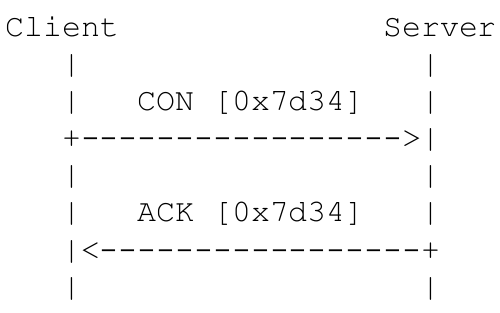
\includegraphics[width=0.5\textwidth]{reliable_message_transmission}
    \caption{Nachrichtenaustausch mit Sicherstellung des Transfers (Quelle: \autocite{RFC7252}).}
    \label{fig:nachrichtenaustausch-mit-sicherstellung-des-transfers}
\end{figure}

Jedoch wird für den Austausch von Nachrichten im CoAP Kontext kein Sicherheitsmechanismus für die Übertragung gefordert, sondern es können auch Nachrichten als \textit{Non-confirmable} markiert werden (siehe Bild \ref{fig:nachrichtenaustausch-ohne-sicherstellung-des-transfers}). Dies bietet sich zum Beispiel an, wenn man die Messdaten eines Sensors wiederholt ausliest. Dabei werden \textit{Non-confirmable} Nachrichten nicht bestätigt, jedoch wird eine \textit{Message ID} benutzt, um Duplikate zu erkennen.

\begin{figure}[h]
    \centering
    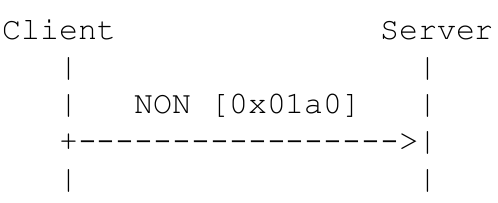
\includegraphics[width=0.5\textwidth]{unreliable_message_transmission}
    \caption{Nachrichtenaustausch ohne Sicherstellung des Transfers (Quelle: \autocite{RFC7252}).}
    \label{fig:nachrichtenaustausch-ohne-sicherstellung-des-transfers}
\end{figure}

\subsubsection{Anfragen/Antwort Modell}
\label{subsubsec:anfragen-antwort-modell}

Kann eine einkommende Anfrage (\textit{Request}), die mithilfe einer \textit{Confirmable} Nachricht versendet wurde, sofort beantwortet werden, wird die Antwort (\textit{Response}) in der daraus resultierenden \textit{Acknowledgment} Nachricht zurückgesendet. Dieses Prinzip nennt man auch \textit{Piggybacked Response}. Das Bild \ref{fig:beispiel-eines-erfolgreichen-piggybacked-response} stellt diesen Mechanismus dar.

\begin{figure}[h]
    \centering
    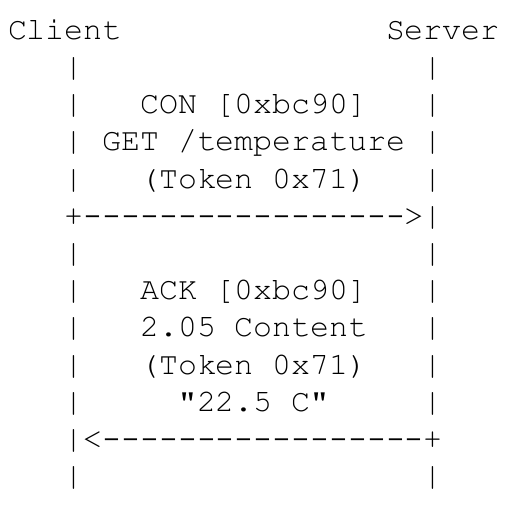
\includegraphics[width=0.5\textwidth]{piggybacked_response}
    \caption{Beispiel eines erfolgreichen \textit{Piggybacked Response} (Quelle: \autocite{RFC7252}).}
    \label{fig:beispiel-eines-erfolgreichen-piggybacked-response}
\end{figure}

Ist der Server jedoch nicht sofort in der Lage die Anfrage zu beantworten, dann antwortet dieser mit einer leeren \textit{Confirmable} Nachricht. Dies tut er, um den Client vom wiederholten Senden der Anfrage zu stoppen. Sind alle benötigten Daten zur Beantwortung der Anfrage vorhanden, sendet der Server die Antwort in einer neuen \textit{Confirmable} Nachricht. Dieses Prinzip wird als separate Antwort (\textit{separate response}) bezeichnet und kann mit dem Bild \ref{fig:beispiel-einer-separate-response} nachvollzogen werden.

\begin{figure}[h]
    \centering
    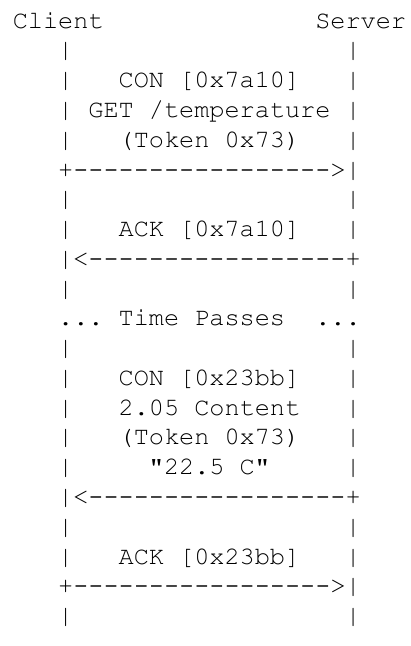
\includegraphics[width=0.5\textwidth]{separate_response}
    \caption{Beispiel einer \textit{separate response} (Quelle: \autocite{RFC7252}).}
    \label{fig:beispiel-einer-separate-response}
\end{figure}

Dabei macht CoAP Gebrauch von den bekannten Internetmethoden \textit{GET}, \textit{PUT}, \textit{POST} und \textit{DELETE} in einer ähnlichen Art wie es HTTP tut.

\subsection{Nachrichtenformat}
\label{subsec:nachrichtenformat}

Wie schon erwähnt, basiert der Nachrichtenaustausch von CoAP auf UDP. Dabei nimmt jede, über UDP versendete Nachricht ein ganzes UDP Datagramm. Dabei ist der Aufbau einer CoAP Nachricht einfach gehalten und startet mit einer Vier-Byte-langen-Kopfzeile (\textit{Header}). Diese beinhaltet folgende Daten (visualisiert im Bild \ref{fig:binaere-sturktur-eines-coap-headers}):
\begin{itemize}
    \item \textit{Version}
    \item \textit{Type}
    \item \textit{Token Length}
    \item \textit{Code}
    \item \textit{Message ID}
\end{itemize}

Dabei repräsentieren die ersten zwei Bits des \textit{Headers} die Versionsnummer. Die Versionsnummer gibt an, welcher CoAP Version die Nachricht erstellt wurde bzw. verarbeitet werden kann. In dieser Arbeit beschäftigen wir uns mit CoAP Nachrichten mit der Versionsnummer 1 (01 in Binär).

Die darauffolgenden zwei Bits entsprechen dem Typ der CoAP Nachricht. Der Typ gibt an, ob es sich um eine \textit{Confirmable} (0 = 00 in Binär), \textit{Non-Confirmable} (1 = 01), \textit{Acknowledgement}  (2 = 10) oder \textit{Reset} (3 = 11) Nachricht handelt.

Als Nächstes kommt die vier Bit lange \textit{Token Length}, die die Länge des \textit{Tokens} angibt. Dabei kann der \textit{Token} zwischen null (0000 in Binär) und acht (0111) Bytes betragen. \textit{Token Lengths} zwischen neun und fünfzehn Bytes sind im RFC 7252 \autocite{RFC7252} für zukünftige Versionen reserviert.

Die nächsten 8 Bit geben den \textit{Code} (vgl. mit dem Statuscode bei HTTP) der CoAP Nachricht an. Dabei unterteilt sich der \textit{Code} in eine drei Bit lange \textit{Code Class} (\textit{most significant bits}) und einen fünf Bit lange \textit{Code Detail} (\textit{least significatn bits}). Dabei folgt der \textit{Code} dem Schema "c.dd", wobei "c" Werte von 0 bis 7 annehmen kann und "dd" Werte von 00 bis 31. Die \textit{Code Class} gibt dabei an, ob es sich um
\begin{itemize}
    \item eine Anfrage (0),
    \item eine erfolgreiche Antwort (2),
    \item eine clientseitige, fehlerhafte Antwort (4),
    \item oder eine serverseitige, fehlerhafte Antwort (5).
\end{itemize}

Dabei nimmt der \textit{Code} 0.00 eine besondere Stellung ein, da dieser eine leere Nachricht (\textit{Empty Message}) markiert. Die \textit{Codes} gleichen sich mit einigen Statuscodes, die man von HTTP kennt, jedoch ist nicht jeder Statuscode als CoAP \textit{Code} abgebildet.

Der letzte Teil des \textit{Headers} ist die sogenannte \textit{Message Id}, die 16 Bit in Anspruch nimmt und in der \textit{Networt Byte Order} (\textit{Big Endian}) angegeben wird. Ihre Aufgabe ist es, Duplikate von Nachrichten zu erkennen. Auch wird die \textit{Message Id} dazu benutzt, um Nachrichten vom Typ \textit{Acknowledgement} und \textit{Reset} zu Nachrichten vom Typ \textit{Confirmable} und \textit{Non-Confirmable} zu verlinken. Somit besitzt der Server immer einen Überblick, zu welcher Anfrage schon eine Antwort geschickt wurde.

\begin{figure}[h]
    \centering
    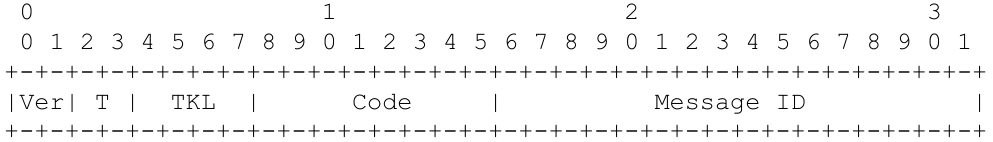
\includegraphics[width=0.75\textwidth]{coap_header}
    \caption{Binäre Struktur eines CoAP \textit{Headers} (Quelle: \autocite{RFC7252}).}
    \label{fig:binaere-sturktur-eines-coap-headers}
\end{figure}

Anschließend an den \textit{Header} kommt der \textit{Token} der Nachricht. Dieser ist in seiner Länge variabel und hängt von der im \textit{Header} angegebenen \textit{Token Length} ab. Dieser ist zuständig für die Korrelation von Anfragen zu Antworten.

Nachfolgend können null oder mehr sogenannten \textit{Options} folgen. Der Option können folgende Bestandteile einer CoAP Nachricht folgen:
\begin{itemize}
    \item das Ende der CoAP Nachricht (EoF),
    \item eine weitere Option,
    \item oder der \textit{Payload Marker} mit anschließender \textit{Payload}.
\end{itemize}

Ist eine \textit{Payload} gegeben, folgt nach der Gruppe von \textit{Options} ein sogenannter \textit{Payload Marker}. Dieser besteht aus einem Byte voller logischer Einsen (0xFF) und markiert somit das Ende der \textit{Options}. Alle Daten, die nach dem \textit{Payload Marker} befinden, werden als \textit{Payload} behandelt. Dabei ist die Länge durch die \textit{UDP Datagram} Paketgröße begrenzt. Wird für die Übertragung der Nachricht mehr Bytes benötigt, als ein \textit{UDP Datagram} an Größe bereitstellen kann, werden die Bytes auf mehrere \textit{UDP Datagrams} aufgespalten. Diesen Mechanismus nennt man auch \textit{Blockwise transfer} und wird im RFC 7959 beschrieben \autocite{RFC7959}.

\begin{figure}[h]
    \centering
    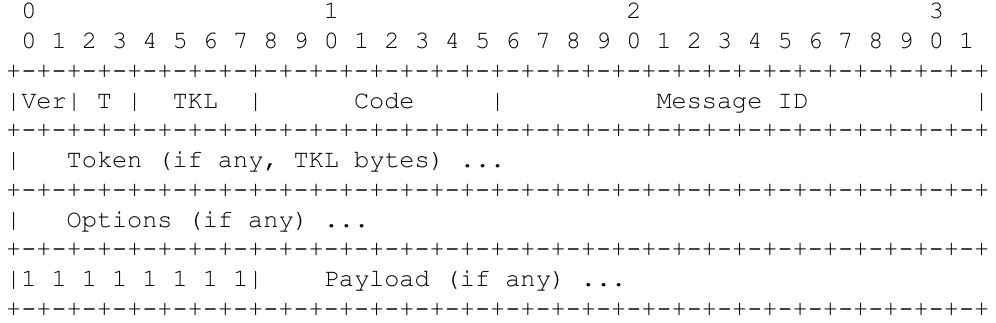
\includegraphics[width=0.75\textwidth]{coap_message}
    \caption{Binäre Struktur einer vollständigen CoAP Nachricht (Quelle: \autocite{RFC7252}).}
    \label{fig:binaere-sturktur-einer-vollstaendigen-coap-nachricht}
\end{figure}

\subsection{Aufbau einer Option}
\label{subsec:aufbau-einer-option}

Eine Option wird durch eine eindeutige Nummer identifiziert. Neben der Nummer besitzt eine Option auch einen Wert (\textit{Value}), den diese Option hält, und einen Indikator für die Länge des Wertes. Dabei wird die Nummer nicht direkt in die Nachricht kodiert, sondern die Options werden zuerst aufsteigend nach ihrer Nummer sortiert und dann wird eine Deltakodierung (Differenzbildung) zwischen der aktuellen Option und deren Vorgängern gebildet. Dies geschieht dadurch, dass alle vorherigen Differenzen (\textit{Deltas}) addiert werden und dann die Differenz zur aktuellen Option gebildet wird. Für die erste Option wird der Sonderfall behandelt, dass als vorheriges Delta ein Wert von null angenommen wird. Dies resultiert darin, dass für die erste Option die kodierte Differenz als Nummer der Option verwendet wird. Ein weiterer Sonderfall ist derjenige, wenn mehrere Instanzen der gleichen Option in der Kollektion von Options auftritt. Dabei ist die Differenz zwischen zwei gleichen Options immer null.

Eine Option fängt immer mit einem Byte an, das zwei Informationen enthält. Einmal die Differenz (\textit{Option Delta}) und die Länge des Wertes (\textit{Option Length}) der Option. Das \textit{Option Delta} entspricht dabei den ersten vier Bits (\textit{most significant bits}) und die \textit{Option Length} die letzten vier Bits (\textit{least significant bits}). Man kann dieses Byte auch als einen \textit{Header} für Options bezeichnen, da dieser Informationen beinhaltet, die für das Kodierung bzw. Dekodieren von Options benötigt wird.

Um jedoch Differenzen und Längen, jenseits des Wertes fünfzehn, verwenden zu können, können dem \textit{Option Header} das \textit{Option Delta (extended)} und \textit{Option Length (extended)} folgen. Diese beiden können jeweils zwischen null und zwei Bytes lang sein. Nach diesen beiden folgt der \textit{Option Value}, der null oder mehr Bytes betragen kann.

\subsubsection{Parsen einer Option}
\label{subsubsec:parsen-einer-option}


